\section{Nodos l\'ogicos del IED IEDRV}
\label{sec:LNs-del-IEDRV}

En la figura \ref{fig:MODEL-resumen-IEDRV} se presenta un resumen
de los nodos l�gicos m�s importantes, y en las tablas a continuaci�n se 
presentan los detalles correspondientes.

Los nodos l�gicos de esta secci�n corresponden
a los IEDs reguladores de velocidad (primaria y secundaria). Los 
IEDs son id�nticos. Simplemente cambian los algoritmos internos 
basados en los nodos l�gicos \textbf{FPID}.

\begin{figure}
\begin{center}
  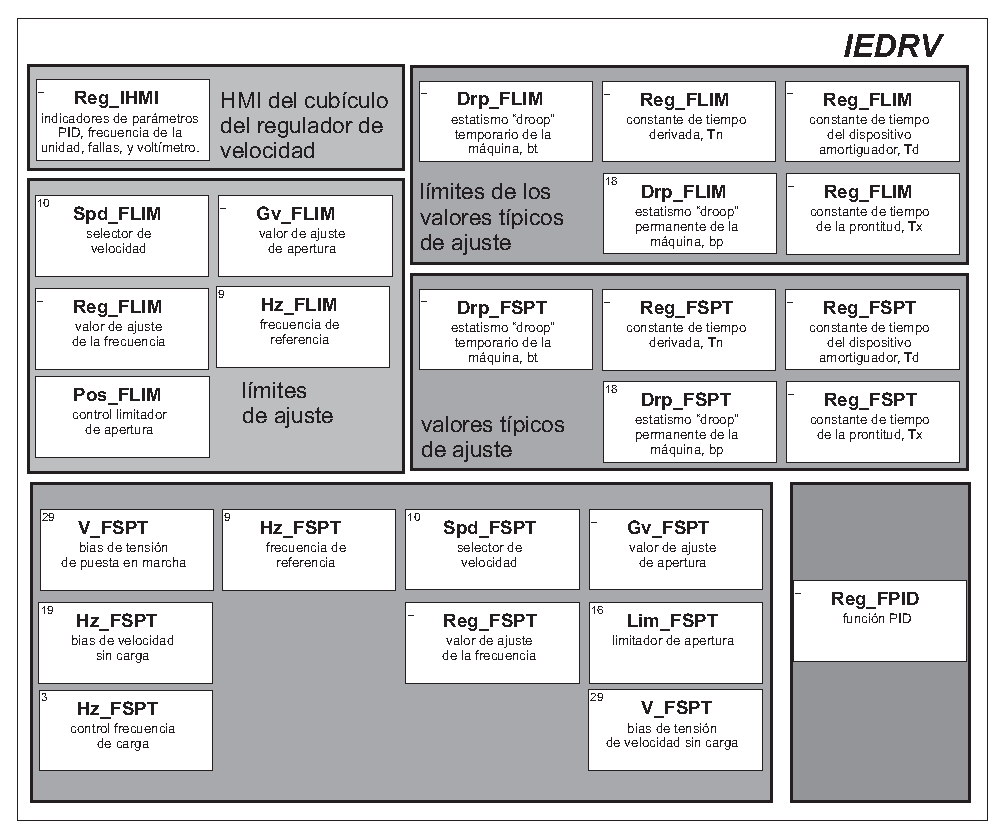
\includegraphics[width=0.7\linewidth]{chapters/model/figures/LN-IEDRV.eps} 
  \caption{Resumen de los nodos l�gicos m�s importantes del IED \emph{IEDRV}}
  \label{fig:MODEL-resumen-IEDRV}
\end{center}
\end{figure}


\subsection{Nodo l\'ogico: 			 FPID}

    \subsubsection{Instancias del nodo l\'ogico FPID}
    \begin{table}[H]
    \begin{center}
    \begin{tabular}{|l|l|p{6.8cm}|}
            \hline
            \multicolumn{3}{|c|}{\cellcolor[gray]{0.8} \textbf{IED Logical Nodes} } \\
            \hline
            \textbf{LN Name} & \textbf{Logical Device Allocation} & \textbf{Code and description} \\
            \hline
            FPID\_reg & LD5 & Funci\'on PID \\			
            \hline
    \end{tabular}
    \caption{Instancias FPID en el IED IEDRV}
    \label{table:lnInstFPID_reg}
    \end{center}
    \end{table}
    
    \lstinputlisting[label=code:scliedFPID,
            caption=Instancias FPID representadas en SCL
            ]{chapters/model/iedE/iedFPID_reg.xml}
    
    \subsubsection{DataTypeTemplate}
    \begin{table}[H]
    \begin{center}
    \begin{tabular}{|l|l|p{8.5cm}|}
            \hline
            \multicolumn{3}{|c|}{\cellcolor[gray]{0.8} \textbf{ FPID}  - PID Function} \\
            \hline
            \textbf{Attribute Name} & \textbf{Attr. Type} & \textbf{Explanation} \\
            \hline 
            Mod & INC & Mode \\
            \hline
            Beh & INS & Behaviour \\
            \hline
            Health & INS & Health \\
            \hline
            NamPlt & LPL & Name plate \\
            \hline
            Out & MV & PID output \\
            \hline
            PAct & MV & Proportional action \\
            \hline
            IAct & MV & Integral action \\
            \hline
            DAct & MV & Derivative action \\
            \hline
            P & MV & P output \\
            \hline
            I & MV & I output \\
            \hline
            D & MV & D output \\
            \hline
    \end{tabular}
    \caption{Plantilla FPID del IED IEDRV}
    \label{table:lnTypeFPID_reg}
    \end{center}
    \end{table}
    
    \lstinputlisting[label=code:sclFPID,
            caption=FPID - PID Function - Representaci\'on en SCL
            ]{chapters/model/iedE/FPID.xml}
     



\subsection{Nodo l\'ogico: 			 FLIM}

    \subsubsection{Instancias del nodo l\'ogico FLIM}
    \begin{table}[H]
    \begin{center}
    \begin{tabular}{|l|l|p{6.8cm}|}
            \hline
            \multicolumn{3}{|c|}{\cellcolor[gray]{0.8} \textbf{IED Logical Nodes} } \\
            \hline
            \textbf{LN Name} & \textbf{Logical Device Allocation} & \textbf{Code and description} \\
            \hline
            Drp\_FLIM1 & LD1 & L\'imites del estatismo DROOP temporario de la m\'aquina \\
            \hline
            Reg\_FLIM2 & LD1 & L\'imites de la constante de tiempo derivada, Tn \\
            \hline
            Reg\_FLIM3 & LD1 & L\'imites de la constante de tiempo del dispositivo amortiguador, Td \\
            \hline
            Drp\_FLIM4 & LD1 & L\'imites del estatismo DROOP permanente de la m\'aquina \\
            \hline
            Reg\_FLIM5 & LD1 & L\'imites de la constante de tiempo de la prontitud, Tx \\
            \hline
            Spd\_FLIM6 & LD2 & L\'imites del selector de velocidad \\
            \hline
            Gv\_FLIM7 & LD2 & L\'imites del valor de ajuste de apertura \\
            \hline
            Reg\_FLIM8 & LD2 & L\'imites del valor de ajuste de la frecuencia \\
            \hline
            Hz\_FLIM9 & LD2 & L\'imites de la frecuencia de referencia \\
            \hline
            Pos\_FLIM10 & LD2 & L\'imites del control limitador de apertura \\
            \hline
    \end{tabular}
    \caption{Instancias FLIM en el IED IEDRV}
    \label{table:lnInstFLIM_tipical}
    \end{center}
    \end{table}
    
    \lstinputlisting[label=code:scliedFLIM,
            caption=Instancias FLIM representadas en SCL
            ]{chapters/model/iedE/iedFLIM_tipical.xml}
    
    \subsubsection{DataTypeTemplate}
    \begin{table}[H]
    \begin{center}
    \begin{tabular}{|l|l|p{8.5cm}|}
            \hline
            \multicolumn{3}{|c|}{\cellcolor[gray]{0.8} \textbf{ FLIM}  - Limits of typical values} \\
            \hline
            \textbf{Attribute Name} & \textbf{Attr. Type} & \textbf{Explanation} \\
            \hline 
            Mod & INC & Mode \\
            \hline
            Beh & INS & Behaviour \\
            \hline
            Health & INS & Health \\
            \hline
            NamPlt & LPL & Name plate \\
            \hline
            HiLim & SPS &   \\
            \hline
            LoLim & SPS &   \\
            \hline
            Out & MV &   \\
            \hline
            HiLimSpt & ASG &   \\
            \hline
            LoLimSpt & ASG &   \\
            \hline
    \end{tabular}
    \caption{Plantilla FLIM del IED IEDRV}
    \label{table:lnTypeFLIM_tipical}
    \end{center}
    \end{table}
    
    \lstinputlisting[label=code:sclFLIM,
            caption=FLIM - Limits of typical values - Representaci\'on en SCL
            ]{chapters/model/iedE/FLIM.xml}
     
  
  

\subsection{Nodo l\'ogico: 			 FSPT}

    \subsubsection{Instancias del nodo l\'ogico FSPT}
    \begin{table}[H]
    \begin{center}
    \begin{tabular}{|l|l|p{6.8cm}|}
            \hline
            \multicolumn{3}{|c|}{\cellcolor[gray]{0.8} \textbf{IED Logical Nodes} } \\
            \hline
            \textbf{LN Name} & \textbf{Logical Device Allocation} & \textbf{Code and description} \\
            \hline
            Drp\_FSPT1 & LD3 & Estatismo DROOP temporario de la m\'aquina \\
            \hline
            Reg\_FSPT2 & LD3 & Constante de tiempo derivada, Tn \\
            \hline
            Reg\_FSPT3 & LD3 & Constante de tiempo del dispositivo amortiguador, Td \\
            \hline
            Drp\_FSPT4 & LD3 & Estatismo DROOP permanente de la m\'aquina \\
            \hline
            Reg\_FSPT5 & LD3 & Constante de tiempo de la prontitud, Tx \\
            \hline
            V\_FSPT6 & LD4 & Bias de tensi\'on de puesta en marcha \\
            \hline
            Hz\_FSPT7 & LD4 & Frecuencia de referencia \\
            \hline
            Spd\_FSPT8 & LD4 & Selector de velocidad \\
            \hline
            Gv\_FSPT9 & LD4 & Valor de ajuste de apertura \\
            \hline
            Hz\_FSPT10 & LD4 & Bias de velocidad sin carga \\
            \hline
            V\_FSPT11 & LD4 & Bias de tensi\'on de velocidad sin carga \\
            \hline
            Lim\_FSPT12 & LD4 & Limitador de apertura \\
            \hline
            Hz\_FSPT13 & LD4 & Control frecuencia de carga \\
            \hline
            Reg\_FSPT14 & LD4 & Valor de ajuste de la frecuencia \\
            \hline
    \end{tabular}
    \caption{Instancias FSPT en el IED IEDRV}
    \label{table:lnInstFSPT_1}
    \end{center}
    \end{table}
    
    \lstinputlisting[label=code:scliedFSPT,
            caption=Instancias FSPT representadas en SCL
            ]{chapters/model/iedE/iedFSPT_1.xml}
    
    \subsubsection{DataTypeTemplate}
    \begin{table}[H]
    \begin{center}
    \begin{tabular}{|l|l|p{8.5cm}|}
            \hline
            \multicolumn{3}{|c|}{\cellcolor[gray]{0.8} \textbf{ FSPT}  - Set point control function} \\
            \hline
            \textbf{Attribute Name} & \textbf{Attr. Type} & \textbf{Explanation} \\
            \hline 
            Mod & INC & Mode \\
            \hline
            Beh & INS & Behaviour \\
            \hline
            Health & INS & Health \\
            \hline
            NamPlt & LPL & Name plate \\
            \hline
            SptMem & MV & Set point in memory \\
            \hline
    \end{tabular}
    \caption{Plantilla FSPT del IED IEDRV}
    \label{table:lnTypeFSPT_1}
    \end{center}
    \end{table}
    
    \lstinputlisting[label=code:sclFSPT,
            caption=FSPT - Set point control function - Representaci\'on en SCL
            ]{chapters/model/iedE/FSPT.xml}
     
  
  
  
  

    